% Angabe zu Blattgröße, Schriftgröße, Hinzufügen des Bildverzeichnis und Quellverzeichnis als Punkt im Inhaltsverzeichnis, einseitiger Druck
\documentclass[a4paper,12pt,listof=toc,bibliography=totoc,oneside, titlepage, headsepline,headings=optiontohead]{scrartcl}	
\usepackage{geometry}
\usepackage[utf8]{inputenc} % Zeichenkodierung
\usepackage[ngerman]{babel} %Sprachpaket
\usepackage{blindtext}
\usepackage{csquotes}
\usepackage{graphicx}
\usepackage{amssymb}
\usepackage{enumitem,xcolor}
\usepackage{xpatch}
%Verlinkungen inner- und außerhalb von Latex
\usepackage[pdftex]{hyperref}
\usepackage[hyperref]{ntheorem}
\usepackage[automark]{scrlayer-scrpage}
\usepackage{titletoc}
%Grafik und Grafikpositionierung
\usepackage{graphicx}
\usepackage{here}
\usepackage[export]{adjustbox}
\usepackage[many]{tcolorbox}
\usepackage{framed}
\usepackage{subfig}
\usepackage[strict]{changepage}
\graphicspath{{img/}}

%-- colorize blindtext--
\LetLtxMacro{\blindtextblindtext}{\blindtext}
\RenewDocumentCommand{\blindtext}{O{\value{blindtext}}}{%
  \begingroup\color{red}\blindtextblindtext[#1]\endgroup
}

%Seitenränder
\geometry{a4paper, top=30mm, left=20mm, right=20mm, bottom=25mm, headsep=10mm, footskip=15mm}

%THM-Farben
\definecolor{thm_green}{cmyk}{0.57,0,1,0}
\definecolor{thm_grey}{cmyk}{0.33, 0.04, 0, 0.72}
\definecolor{thm_red}{cmyk}{0, 1, 0.65, 0.28}
\definecolor{thm_yellow}{cmyk}{0,0.30,1,0}
\definecolor{thm_lightblue}{cmyk}{0.75,0,0.07,0}
\definecolor{thm_blue}{cmyk}{0.1,0.72,0,0.18}
\definecolor{thm_lightGray}{cmyk}{0.07,0,0,0.12}

% Kopf - und Fusszeile
\clearpairofpagestyles
\ihead{\leftmark}
\addtokomafont{headsepline}{\color{thm_green}}
\cfoot*{\pagemark}

%=========== Zitate ===========================================================%

\newenvironment{formal}{%
  \def\FrameCommand{%
    \hspace{1pt}%
    {\color{thm_grey}\vrule width 5pt}%
    {\color{thm_grey!10}\vrule width 4pt}%
    \colorbox{thm_grey!10}%
  }%
  \MakeFramed{\advance\hsize-\width\FrameRestore}%
  \noindent\hspace{-4.55pt}% disable indenting first paragraph
  \begin{adjustwidth}{}{7pt}%
  \vspace{2pt}\vspace{2pt}%
}
{%
  \vspace{2pt}\end{adjustwidth}\endMakeFramed%
}

%===== Bildherkunft =========================
\newcommand{\captionsource}[1]{\itshape\footnotesize (#1)}

% Deckblatt
\makeatletter
\AtBeginDocument{\hypersetup{
	pdftitle={\@title},
	% pdfsubject={\@subtitle},
	% pdfauthor={\@author},
	bookmarksopen=true,
	bookmarksopenlevel=3,
	breaklinks,
	colorlinks,
	citecolor=red,
	linkcolor=black,
	urlcolor=black,
}}

\newcommand*{\institute}[1]{\gdef\@institute{#1}}
\newcommand*{\@institute}{}%

\newcommand*{\mail}[1]{\gdef\@mail{#1}}
\newcommand*{\@mail}{}%

\renewcommand*{\maketitle}{%
  \global\@topnum=\z@
  \setparsizes{\z@}{\z@}{\z@\@plus 1fil}\par@updaterelative
  \null
  \vskip 4em%
  \begin{center}%
    \ifx\@subject\@empty \else
      {\usekomafont{subject}{\@subject \par}}%
      \vskip 1.5em
    \fi
    {\usekomafont{title}{\huge \@title \par}}%
    \vskip .5em
    {\ifx\@subtitle\@empty\else\usekomafont{subtitle}\@subtitle\par\fi}%
    \vskip 1em
    {%
      \usekomafont{author}{%
        \lineskip .5em%
        \begin{tabular}[t]{@{}l}
          \@author
        \end{tabular}\par
      }%
    }%
	{\texttt\@mail\par}
    \vfill
    {\usekomafont{publishers}{\@publishers \par}}%
	\vfill
    {\usekomafont{publishers}{\large\@date\\Mathematik, Naturwissenschaften und Informatik\\Technische Hochschule Mittelhessen, Gießen \par}}
  \end{center}%
  \par
  \vskip 2em
}%


\makeatother

\subject{Ausarbeitung}
\title{Projekt E: Forward Collision Avoidance Assist}
\subtitle{Fahrerassistenzsysteme II2511}
\author{Berkay Özgür, C. Arda Sengenc}
\mail{berkay.oezguer@mni.thm.de\\cagkan.arda.sengenc@mni.thm.de}
\publishers{Dozent:\\Prof. Dr.-Ing. Seyed Eghbal Ghobadi}
\institute{Mathematik, Naturwissenschaften und Informatik}


% % % % % % % % % % % % % %
% % % Dokument Beginn % % %
% % % % % % % % % % % % % %
\begin{document}
	%Deckblatt
	\begin{titlepage}
	\begin{minipage}[t]{\textwidth}
		\vspace{-1cm}
		
\includegraphics[height=15mm,valign=t]{thm-logo.pdf}
		\hspace{6mm}
		
\includegraphics[height=10.4mm,valign=t]{mni_2023.png}
	  \end{minipage}
	\maketitle
\end{titlepage}
	
	%Inhaltsverzeichnis
	\pagenumbering{roman}
	\tableofcontents
	\clearpage
	
	%Inhalt
	\pagenumbering{arabic}
	\pagestyle{scrheadings}
	\setcounter{page}{1} %Seitenzähler auf 1 setzen, da Inhaltsverzeichnis sonst als Seite 1 zählt
	\section{Einleitung}
Die Collision Avoidance Assistance ist eine Forschungs- und Entwicklungsinitiative, die darauf abzielt, ein fortschrittliches System zu entwickeln, was die Sicherheit des Fahrers durch Warnungen und autonomes Eingreifen erhöht, um potenzielle Kollisionen zu verhindern. Diese Dokumentation gibt einen Überblick über das Projekt, einschließlich seiner Ziele, Schlüsselkomponenten und Funktionalitäten.

\subsection{Zielsetzung}
Die Hauptziele des Kollisionsvermeidungs-Assistenzprojekts sind wie folgt:
\begin{itemize}
	\item Erhöhung der Sicherheit des Fahrers durch Erkennung und Vermeidung potenzieller Kollisionsszenarien.
	\item Rechtzeitige und genaue Warnungen, um den Fahrer vor möglichen Gefahren zu warnen.
	\item Falls erforderlich, autonom durch Bremsen oder Lenken eingreifen, um Kollisionen zu vermeiden.
	\item Nutzung verschiedener Sensoren, wie Radar, Kamera oder LiDAR, um die Umgebung zu überwachen und potenzielle Kollisionsrisiken zu erkennen.
	\item Entwicklung eines robusten und zuverlässigen Systems, das unter verschiedenen Fahrbedingungen effektiv arbeiten kann.
\end{itemize}

\subsection{System-Vision}
Unsere Vision ist es, ein zuverlässiges Collision Avoidance Assist-System zu entwickeln, das durch Sensoren potenzielle Kollisionen frühzeitig erkennt und den Fahrer alarmiert oder autonom eingreift, um Unfälle zu verhindern. Das Ziel ist es, die Verkehrssicherheit zu erhöhen und das Unfallrisiko zu reduzieren.

	\section{Anforderungsanalyse}
Im Rahmen der Anforderungsanalyse und in Abstimmung mit dem Stakeholder haben wir folgende Funktionale- und nicht-funktionale Anforderungen für das Collision Avoidance Assist-System ermittelt.
Funktionale Anforderungen:
\begin{enumerate}
	\item System-ein- und -ausschaltung: Das System muss über einen speziellen Button im Fahrzeug ein- und ausgeschaltet werden können. Der Fahrer soll die Möglichkeit haben, das System nach Bedarf zu aktivieren oder zu deaktivieren.
	\item Mindestgeschwindigkeit: Das System soll erst ab einer Mindestgeschwindigkeit von 10 km/h aktiv werden. Unter dieser Geschwindigkeit bleibt das System inaktiv, um unnötige Warnungen oder Eingriffe zu vermeiden.
	\item Safety Distance Berechnung: Das System muss in der Lage sein, die Sicherheitsabstände zwischen dem eigenen Fahrzeug und vorausfahrenden Fahrzeugen zu berechnen. Basierend auf diesen Abständen soll das System potenzielle Kollisionsszenarien frühzeitig erkennen und den Fahrer entsprechend warnen oder autonom eingreifen.
\end{enumerate}
Nicht-funktionale Anforderungen:
\begin{enumerate}
	\item Zuverlässigkeit: Das System muss zuverlässig und fehlerfrei funktionieren, um die Sicherheit der Fahrzeuginsassen und anderer Verkehrsteilnehmer zu gewährleisten.
	\item Reaktionszeit: Das System muss schnell auf Änderungen in der Umgebung reagieren und innerhalb von Millisekunden Warnungen oder Eingriffe ausführen, um Unfälle zu vermeiden.
	\item Benutzerfreundlichkeit: Die Benutzeroberfläche zur Aktivierung und Deaktivierung des Systems muss intuitiv und einfach zu bedienen sein, um eine fehlerfreie Handhabung zu ermöglichen.
	\item Datenschutz und Sicherheit: Das System muss die Privatsphäre der Fahrzeuginsassen respektieren und sensible Daten sicher verarbeiten. Es darf keine unerlaubte Datenweitergabe oder unbefugten Zugriff ermöglichen.
\end{enumerate}
\subsection{Use Cases - Szenarien}
\begin{table}[H]
	\centering
	\begin{tabular}{| c | p{11cm} |}
		\hline
		\textbf{Abschnitt} & \textbf{Beschreibung}\\
		\hline
		Name & Forward Collision Warning\\
		\hline
		Primärer Akteur & Collision Avoidance Assist System\\
		\hline
		Weitere Akteure & Fahrer\\
		\hline
		Stakeholder Ziele & Vermeidung von Auffahrunfällen, Erhöhung der Verkehrssicherheit\\
		\hline
		Auszulösendes Ereignis & Das vorausfahrende Fahrzeug bremst plötzlich oder verlangsamt sich stark.\\
		\hline
		Beschreibung & Das System warnt den Fahrer vor einer möglichen Kollision, wenn das Fahrzeug zu nahe an einem vorausfahrenden Fahrzeug ist.\\
		\hline
		Vorbedingung & Das Collision Avoidance Assist-System ist aktiviert und einsatzbereit.\\
		\hline
		Nachbedingung & Der Fahrer wird über die mögliche Kollision informiert.\\
		\hline
		Hauptszenario & 1.1. Das System überwacht kontinuierlich den Abstand zum vorausfahrenden Fahrzeug und die Relativgeschwindigkeit. \newline
						1.2. Wenn der Abstand kritisch wird und eine Kollision droht, sendet das System eine visuelle oder akustische Warnung an den Fahrer. \newline
						1.3 Der Fahrer kann entsprechend reagieren und die Geschwindigkeit reduzieren, um eine Kollision zu verhindern.\\
		\hline
	\end{tabular}
\end{table}
\begin{table}[H]
	\centering
	\begin{tabular}{| c | p{11cm} |}
		\hline
		\textbf{Abschnitt} & \textbf{Beschreibung}\\
		\hline
		Name & Automatic Emergency Braking\\
		\hline
		Primärer Akteur & Collision Avoidance Assist System\\
		\hline
		Weitere Akteure & Fahrer\\
		\hline
		Stakeholder Ziele & Vermeidung von Kollisionen, Erhöhung der Verkehrssicherheit\\
		\hline
		Auszulösendes Ereignis & Das vorausfahrende Fahrzeug bremst plötzlich, fährt langsamer als uns und es besteht eine akute Kollisionsgefahr.\\
		\hline
		Beschreibung & Das System führt autonom eine Notbremsung durch, um eine Kollision mit dem vorausfahrenden Fahrzeug zu verhindern.\\
		\hline
		Vorbedingung & Das Collision Avoidance Assist-System ist aktiviert und einsatzbereit.\\
		\hline
		Nachbedingung & Das Fahrzeug wird rechtzeitig gestoppt, um eine Kollision zu verhindern.\\
		\hline
		Hauptszenario & 1.1. Das System überwacht kontinuierlich den Abstand zum vorausfahrenden Fahrzeug und die Relativgeschwindigkeit. \newline
		1.2. Wenn der Abstand kritisch wird und eine Kollision droht, initiert das System automatisch eine Notbremsung. \newline
		1.3. Der Fahrer wird über die Notbremsung informiert und kann den Eingriff abbrechen, falls erforderlich. \newline
		1.4. Das Fahrzeug wird rechtzeitig gestoppt, um eine Kollision mit dem vorausfahrenden Fahrzeug zu verhindern.\\
		\hline
	\end{tabular}
\end{table}
\begin{table}[H]
	\centering
	\begin{tabular}{| c | p{11cm} |}
		\hline
		\textbf{Abschnitt} & \textbf{Beschreibung}\\
		\hline
		Name & Automatic Obstacle Avoidance\\
		\hline
		Primärer Akteur & Collision Avoidance Assist System\\
		\hline
		Weitere Akteure & Fahrer\\
		\hline
		Stakeholder Ziele & Vermeidung von Kollisionen mit Hindernissen auf der Fahrbahn\\
		\hline
		Auszulösendes Ereignis & Ein plötzlich auftretendes Hindernis blockiert den Fahrweg.\\
		\hline
		Beschreibung & Das System führt automatisch eine Lenkung durch, um das Hindernis sicher zu umfahren.\\
		\hline
		Vorbedingung & Das Collision Avoidance Assist-System ist aktiviert und einsatzbereit.\\
		\hline
		Nachbedingung & Das Fahrzeug ist sicher an dem Hindernis vorbeigefahren und eine Kollision wurde erfolgreich vermieden. \\
		\hline
		Hauptszenario & 1.1. Das System überwacht kontinuierlich die Umgebung des Fahrzeugs. \newline
		1.2. Wenn ein Hindernis plötzlich auf der Fahrbahn auftaucht und eine Kollision droht, erkennt das System die Gefahr und initiiert das Ausweichmanöver. \newline
		1.3. Das System berechnet eine geeignete Ausweichroute, die sicher an dem Hindernis vorbeiführt und gleichzeitig den Verkehrsregeln und -bedingungen entspricht. \newline
		1.4. Das System führt das Ausweichmanöver durch, indem es autonom die Lenkung und die Geschwindigkeit des Fahrzeugs kontrolliert. \newline 
		1.5. Das Fahrzeug ist sicher an dem Hindernis vorbeigefahren, und eine Kollision wurde erfolgreich vermieden.\\
		\hline
	\end{tabular}
\end{table}

\subsection{Systemarchitektur}
Die Systemarchitektur des Collision Avoidance Assist-Systems basiert auf einem zentralen Simulink-Modell, das alle relevanten Use Cases abdeckt. Dieses Modell ist verantwortlich für die Verarbeitung der von den Sensoren erfassten Daten sowie die Entscheidungsfindung zur Kollisionsvermeidung. Das Simulink-Modell setzt sich aus verschiedenen Blöcken und Algorithmen zur Datenverarbeitung und -analyse zusammen. Es empfängt kontinuierlich Informationen von den Sensoren, die die Umgebung des Fahrzeugs überwachen. \newline
Die Eingabeelemente des Simulink-Modells sind:
\begin{figure}[H]
	\centering	
	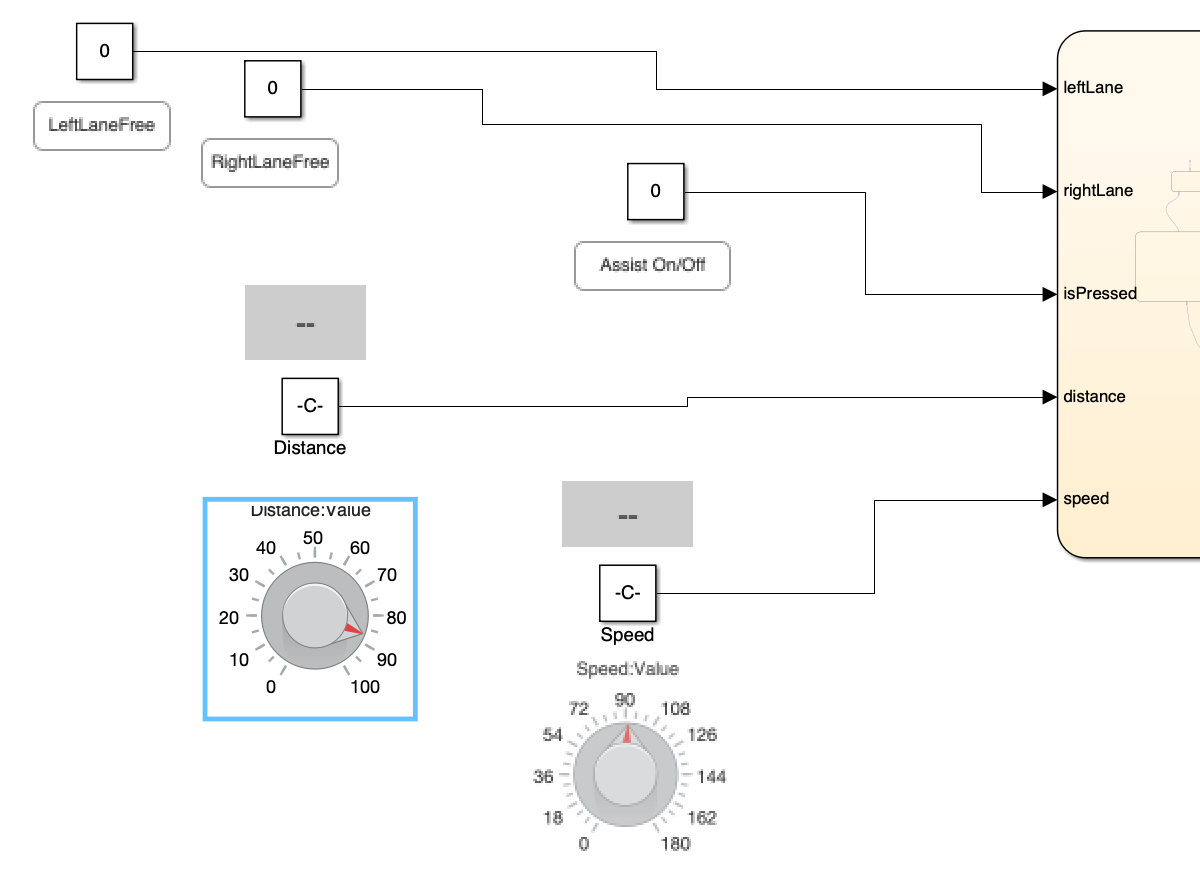
\includegraphics[width=.8\textwidth]{img/eingabeelemente}
	\caption[Eingabeelemente]{Eingabeelemente}
	\label{fig:Eingabeelemente des Simulink-Modells}
\end{figure}
\begin{enumerate}
	\item Buttons für die rechte und linke Spur: Diese Buttons geben an, ob die angrenzenden Fahrspuren frei sind und ob das Fahrzeug ein Ausweichmanöver machen kann.
	\item Ein Button zum Ein- und Ausschalten des Systems: Mit diesem Button kann der Fahrer das Collision Avoidance Assist-System aktivieren oder deaktivieren.
	\item Drehknöpfe für Geschwindigkeit und Abstand: Diese Drehknöpfe ermöglichen es dem Fahrer, die gewünschte Geschwindigkeit des Fahrzeugs und den gewünschten Abstand zum vorausfahrenden Fahrzeug einzustellen.
\end{enumerate}
Die Ausgabeelemente des Simulink-Modells sind:
\begin{figure}[H]
	\centering	
	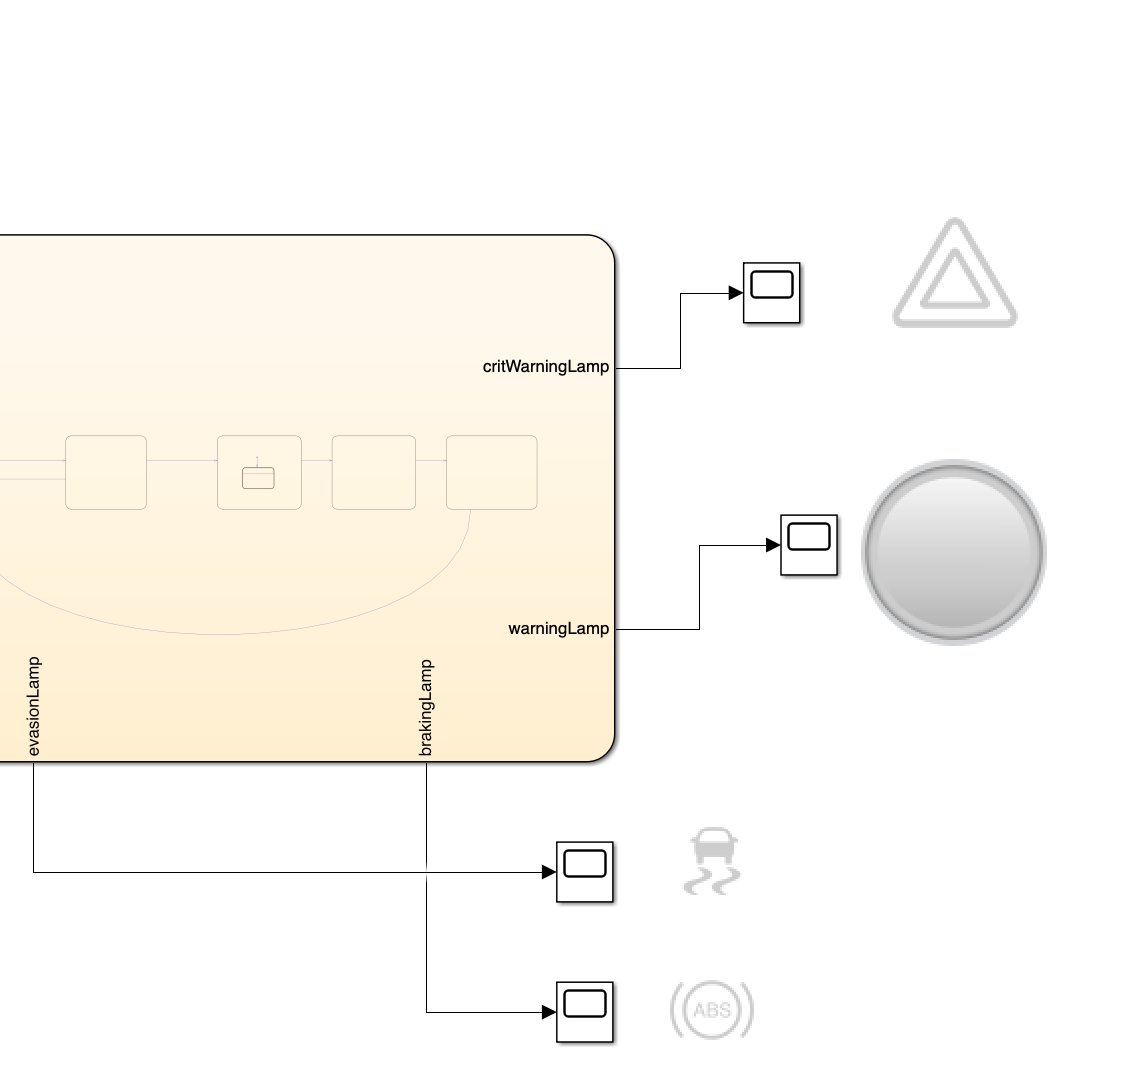
\includegraphics[width=.8\textwidth]{img/ausgabeelemente}
	\caption[Ausgabeelemente]{Ausgabeelemente}
	\label{fig:Ausgabeelemente des Simulink-Modells}
\end{figure}
\begin{enumerate}
	\item Warning Lampe: Diese Lampe leuchtet auf, wenn das System eine potenzielle Kollisionsgefahr erkannt hat und den Fahrer warnt, dass er eingreifen muss.
	\item Critical Warning Lampe: Diese Lampe leuchtet auf, wenn das System eine akute Kollisionsgefahr erkannt hat und eine sofortige Reaktion des Fahrers oder des Systems erforderlich ist, um einen Unfall zu verhindern.
	\item Notfallbremsen Lampe: Diese Lampe leuchtet auf, wenn das System ein Notfallbremsmanöver durchführt, um eine Kollision zu verhindern.
	\item Ausweichmanöver Lampe: Diese Lampe leuchtet auf, wenn das System ein Ausweichmanöver einleitet, um eine Kollision zu vermeiden.
\end{enumerate}
Die Systemarchitektur des Collision Avoidance Assist-Systems umfasst einen Superzustand mit insgesamt sechs Unterzuständen, die den Zustand des Systems während des Betriebs widerspiegeln.
\begin{figure}[H]
	\centering	
	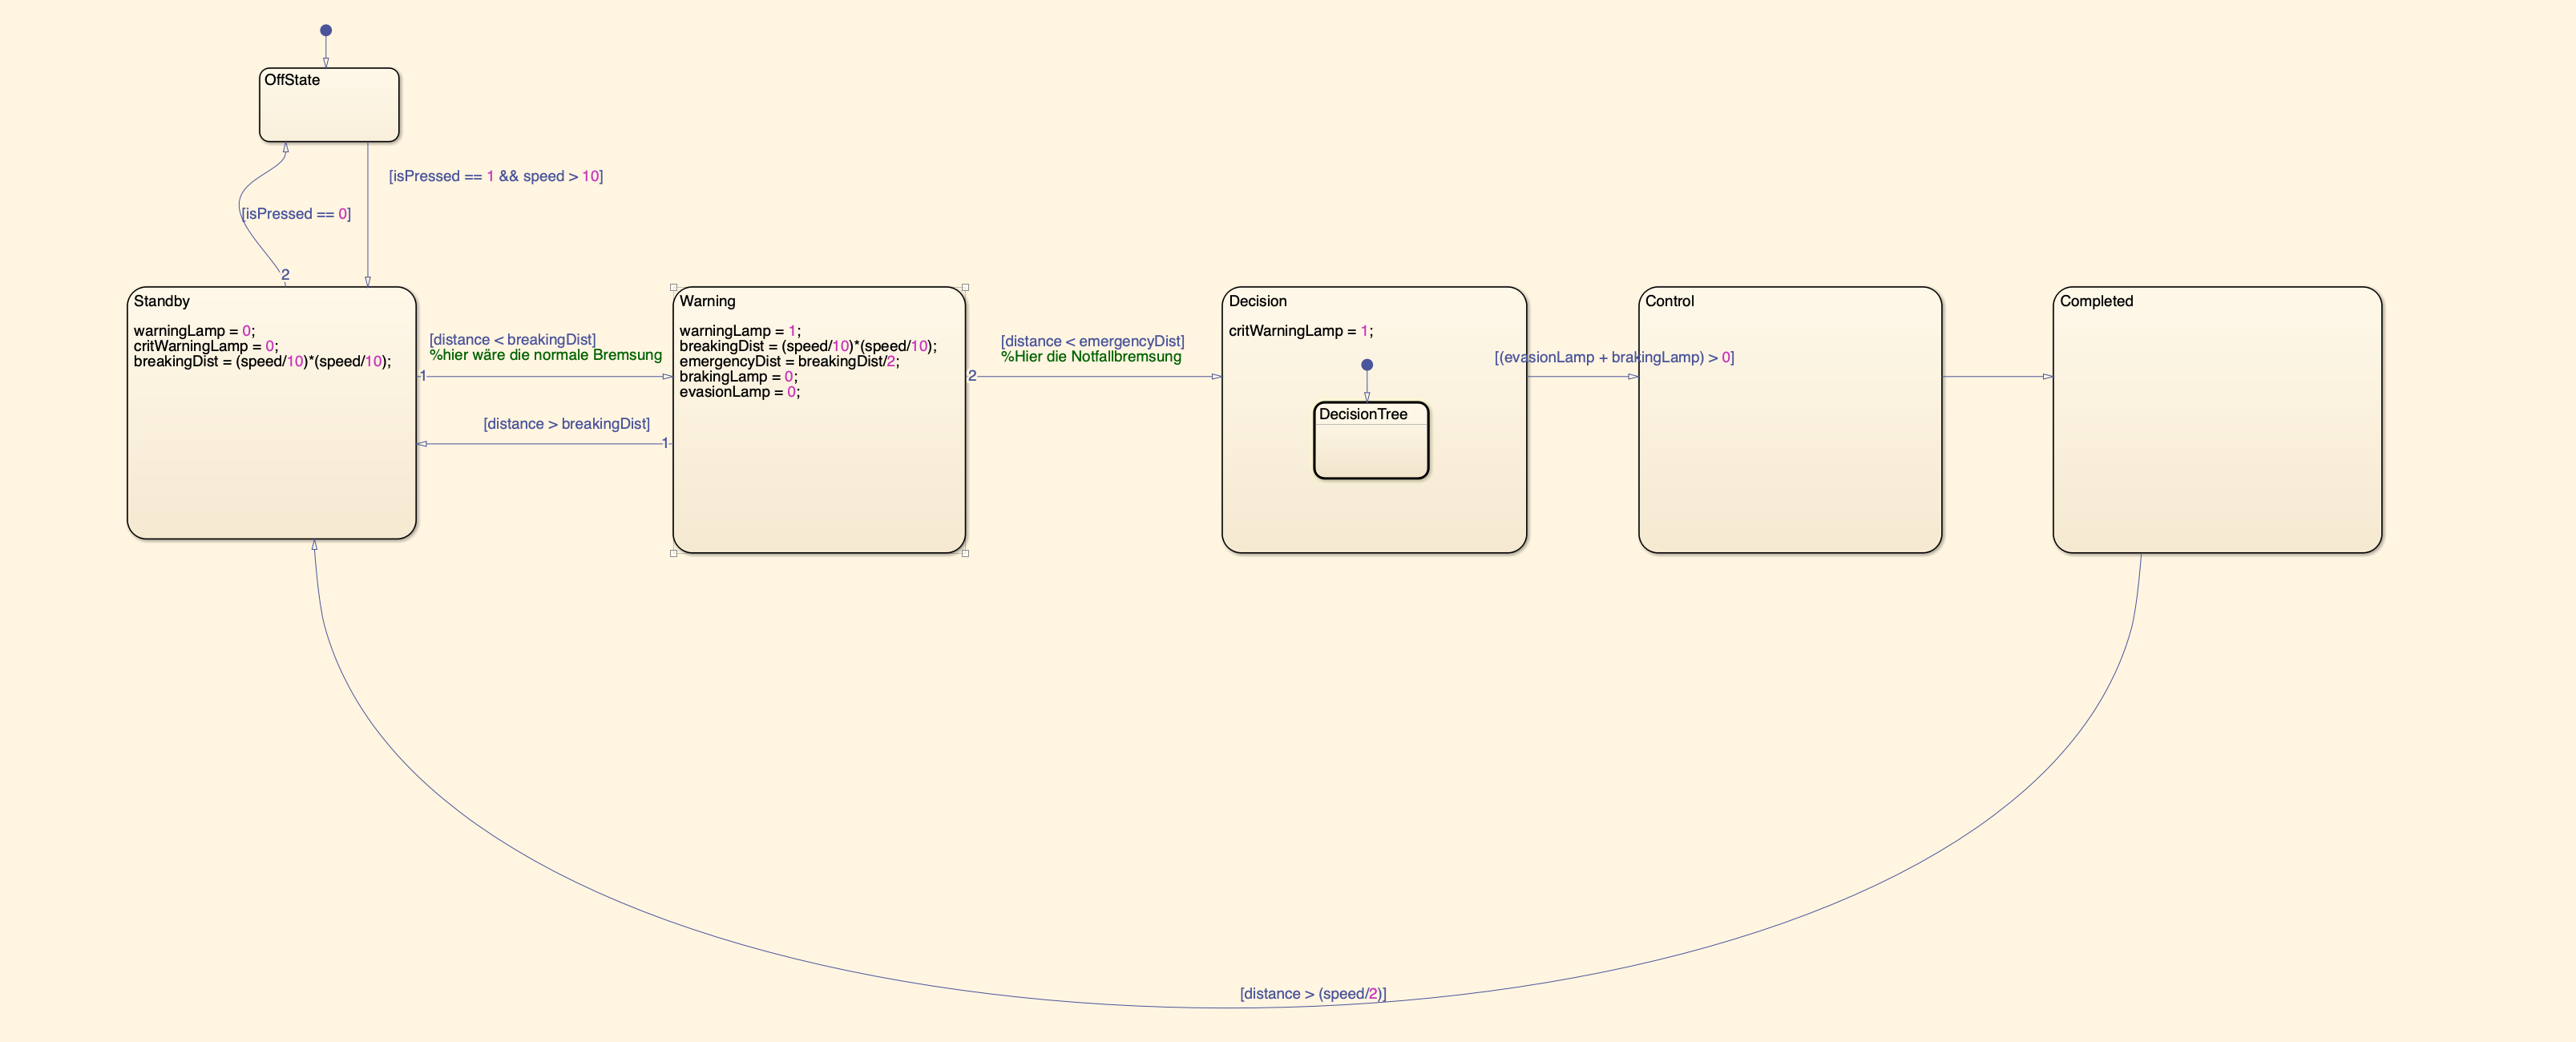
\includegraphics[width=1.0\textwidth]{img/zustaende}
	\caption[Zustände]{Zustände des Systems}
	\label{fig:Zustände des Simulink-Modells}
\end{figure}
\begin{enumerate}
	\item OffState: In diesem Zustand befindet sich das System, wenn es nicht eingeschaltet ist. In diesem Modus werden keine Kollisionsvermeidungsfunktionen aktiviert, und das System bleibt inaktiv.
	\item StandBy: Sobald das System aktiviert ist, wechselt es in den StandBy-Zustand. Hier arbeitet das System, überwacht die Umgebung, erkennt potenzielle Kollisionsszenarien, hat jedoch noch keine Gefahr erkannt.
	\item Warning: Wenn das System eine potenzielle Kollisionsgefahr erkennt, wechselt es in den Warning-Zustand. In diesem Zustand wird die Warning Lampe aktiviert, um den Fahrer über die erkannte Gefahr zu informieren.
	\item Decision: Im Decision-Zustand trifft das System eine kritische Entscheidung, ob eine sofortige Reaktion erforderlich ist, um eine Kollision zu verhindern. Es wird überprüft, ob das Fahrzeug gebremst werden muss oder ein Ausweichmanöver eingeleitet werden sollte.
	\begin{figure}[H]
		\centering	
		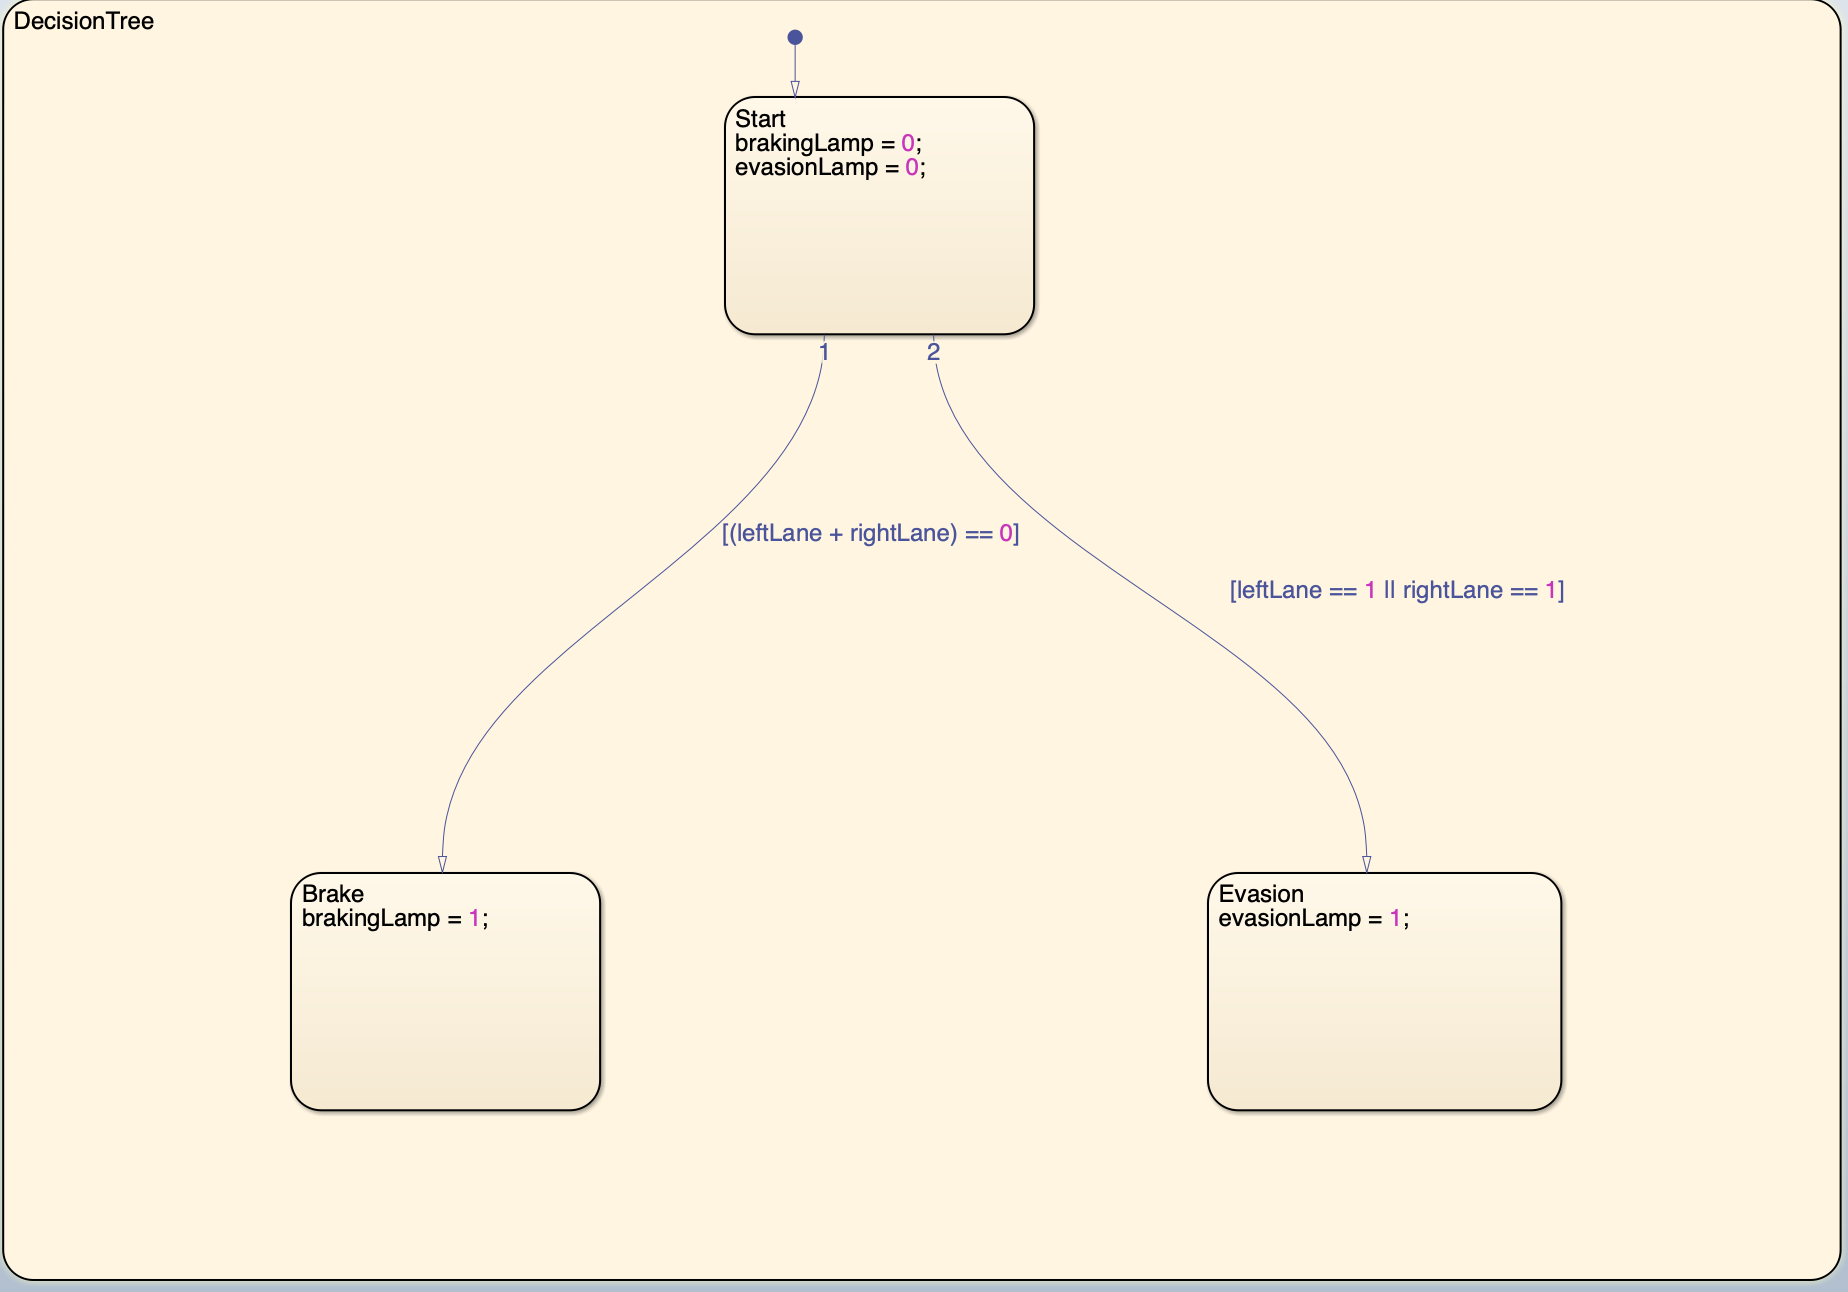
\includegraphics[width=.8\textwidth]{img/entscheidung}
		\caption[Zustände]{Entscheidungsmechanismus}
		\label{fig:Unterzustände von DecisionTree}
	\end{figure}
	\begin{itemize}
		\item Brake: Wenn das System entscheidet, dass ein Notfallbremsmanöver erforderlich ist, wird es in den Brake-Unterzustand wechseln.
		\item Evasion: Wenn das System entscheidet, dass ein Ausweichmanöver erforderlich ist, wird es in den Evasion-Unterzustand wechseln.
	\end{itemize}
	\item Control: In diesem Zustand werden die notwendigen Steuerungseingriffe durchgeführt, um das Notfallbremsmanöver oder das Ausweichmanöver zu realisieren und die potenzielle Kollision zu vermeiden.
	\item Completed: Nachdem das System das Notfallbremsmanöver oder das Ausweichmanöver erfolgreich durchgeführt hat, wechselt es in den Completed-Zustand. Hier wird die Critical Warning Lampe deaktiviert, da die Gefahr erfolgreich vermieden wurde.
\end{enumerate}

\section{Softwareentwurf} % Bitte sinnvolle Überschriften für alle Kapitel und Unterkapitel wählen
\subsection{\enquote{Das Fahrzeug fährt langsam vor uns}}
Diese Funktionalität ist darauf ausgelegt, das Verhalten des Ego-Fahrzeugs zu steuern, wenn es einem langsamer fahrenden Fahrzeug (Bremsfahrzeug) folgt. Das Programm passt die Geschwindigkeit des Ego-Fahrzeugs basierend auf dem Abstand zwischen dem Ego-Fahrzeug und dem Bremsfahrzeug an. \newline
\textbf{Komponenten:}
\begin{enumerate}
	\item Hauptschleife (Main Loop):
	\begin{itemize}
		\item Die Hauptsteuerschleife des Programms, die unendlich läuft.
		\item Ruft Daten von dem Ego-Fahrzeug und dem Bremsfahrzeug (Akteure) ab und berechnet erforderliche Werte.
		\item Bestimmt, ob das Ego-Fahrzeug weiterfahren soll oder eine Bremsung einleiten muss.
		\item Wendet entsprechende Steuersignale (Gaspedal und Bremse) auf das Ego-Fahrzeug an.
		\item Überwacht die vergangene Zeit, um die Simulation nach einer bestimmten Dauer zu beenden.
	\end{itemize}
	\item Algorithmus:
	\begin{itemize}
		\item Platziere das Ego-Fahrzeug und das Bremsfahrzeug an vordefinierten Positionen auf der Straße.
		\item Betrete die Hauptschleife:
		\begin{enumerate}
			\item Erhalte die aktuelle Geschwindigkeit des Ego-Fahrzeugs und berechne die Bremsstrecke und Notbremsstrecke basierend auf der Geschwindigkeit.
			\item Berechne den Abstand zwischen dem Ego-Fahrzeug und dem Bremsfahrzeug.
			\item Steuere das Bremsfahrzeug (Tesla), damit es mit etwas Gas vorwärts fährt.
			\item Prüfe, ob der Abstand zum Bremsfahrzeug kleiner als die Bremsstrecke ist:
			\begin{itemize}
				\item Wenn ja, prüfe, ob der Abstand kleiner als die Notbremsstrecke ist:
				\begin{itemize}
					\item Wenn ja, leite eine Notbremsung ein.
					\item Wenn nein, fahre weiter.
				\end{itemize}
			\end{itemize}
			\item Überwache die vergangene Zeit und beende die Simulation nach einer bestimmten Dauer.
			\item Wiederhole die Schleife, bis die angegebene Zeitdauer erreicht ist.
		\end{enumerate}
	\end{itemize}
\end{enumerate}
\subsection{\enquote{Das Fahrzeug stoppt vor uns}}
Diese Funktionalität ist darauf ausgelegt, das Verhalten des Ego-Fahrzeugs zu steuern, wenn es erkennt, dass das Bremsfahrzeug vor ihm angehalten hat. Das Programm führt Notbremsung ein, um eine Kollision mit dem stehenden Fahrzeug zu vermeiden.\newline
\textbf{Komponenten:}
\begin{enumerate}
	\item Hauptschleife (Main Loop):
	\begin{itemize}
		\item Die Hauptsteuerschleife des Programms, die unendlich läuft.
		\item Ruft Daten von dem Ego-Fahrzeug und dem Bremsfahrzeug (Akteure) ab und berechnet erforderliche Werte.
		\item Bestimmt, ob das Ego-Fahrzeug weiterfahren soll oder eine Bremsung einleiten muss.
		\item Wendet entsprechende Steuersignale (Gaspedal und Bremse) auf das Ego-Fahrzeug an.
		\item Überwacht die vergangene Zeit, um die Simulation nach einer bestimmten Dauer zu beenden.
	\end{itemize}
	\item Algorithmus:
	\begin{itemize}
		\item Platziere das Ego-Fahrzeug und das stehende Fahrzeug an vordefinierten Positionen auf der Straße.
		\item Betrete die Hauptschleife:
		\begin{enumerate}
			\item Erhalte die aktuelle Geschwindigkeit des Ego-Fahrzeugs und berechne die Bremsstrecke und Notbremsstrecke basierend auf der Geschwindigkeit.
			\item Berechne den Abstand zwischen dem Ego-Fahrzeug und dem stehenden Fahrzeug.
			\item Prüfe, ob der Abstand zum Fahrzeug kleiner als die Bremsstrecke ist:
			\begin{itemize}
				\item Wenn ja, prüfe, ob der Abstand kleiner als die Notbremsstrecke ist:
				\begin{itemize}
					\item Wenn ja, leite eine Notbremsung ein.
					\item Wenn nein, fahre weiter.
				\end{itemize}
			\end{itemize}
			\item Überwache die vergangene Zeit und beende die Simulation nach einer bestimmten Dauer.
			\item Wiederhole die Schleife, bis die angegebene Zeitdauer erreicht ist.
		\end{enumerate}
	  	\item Eine graphische Darstellung:
	  	\begin{figure}[H]
	  		\centering	
	  		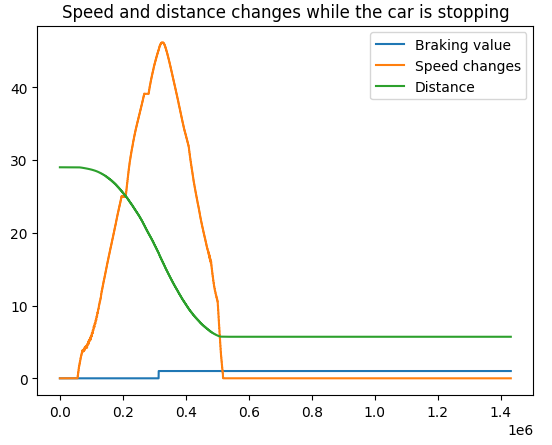
\includegraphics[width=.7\textwidth]{img/stopping_car}
	  		\caption[Notfallbremsung]{Werte einer Notfallbremsung}
	  		\label{fig:notfallbremsung}
	  	\end{figure}
	\end{itemize}
\end{enumerate}
\subsection{\enquote{Ausweichmanöver}}
Diese Funktionalität ist darauf ausgelegt, ein Ausweichmanöver für das Ego-Fahrzeug durchzuführen, wenn sich ein Hindernis oder ein Bremsfahrzeug direkt vor ihm befindet. Das Programm verwendet einen PID-Regler, um das Ego-Fahrzeug sicher um das Hindernis herumzulenken und eine Kollision zu vermeiden. \newline
\textbf{Komponenten:}
\begin{enumerate}
	\item Hauptschleife (Main Loop):
	\begin{itemize}
		\item Die Hauptsteuerschleife des Programms, die unendlich läuft.
		\item Ruft Daten von dem Ego-Fahrzeug und dem Hindernis/Bremsfahrzeug (Akteure) ab und berechnet erforderliche Werte.
		\item Berechnet den gewünschten Steuerwinkel (Steer) für das Ego-Fahrzeug, um das Ausweichmanöver auszuführen.
		\item Steuert das Ego-Fahrzeug entsprechend des berechneten Steuerwinkels.
		\item Überwacht die vergangene Zeit, um die Simulation nach einer bestimmten Dauer zu beenden.
	\end{itemize}
	\item Algorithmus:
	\begin{itemize}
		\item Initialisiere den PID-Regler mit optimalen PID-Verstärkungen Kp, Ki, Kd und der Abtastzeit (dt).
		\item Platziere das Ego-Fahrzeug und das stehende Fahrzeug an vordefinierten Positionen auf der Straße.
		\item Betrete die Hauptschleife:
		\begin{enumerate}
			\item Erhalte die aktuelle Geschwindigkeit des Ego-Fahrzeugs und berechne die Bremsstrecke und Notbremsstrecke basierend auf der Geschwindigkeit.
			\item Berechne den Abstand zwischen dem Ego-Fahrzeug und dem Hindernis/Bremsfahrzeug.
			\item Berechne den gewünschten Steuerwinkel (Steer) für das Ego-Fahrzeug basierend auf der Abstandsregelung (z. B. PID-Regelung).
			\item Steuere das Ego-Fahrzeug entsprechend des berechneten Steuerwinkels.
			\item Überwache die vergangene Zeit und beende die Simulation nach einer bestimmten Dauer.
			\item Wiederhole die Schleife, bis die angegebene Zeitdauer erreicht ist.
		\end{enumerate}
		\item Eine graphische Darstellung:
		\begin{figure}[H]
			\centering
			\subfloat[\centering Anpassen der X-Koordinaten des Autos]{{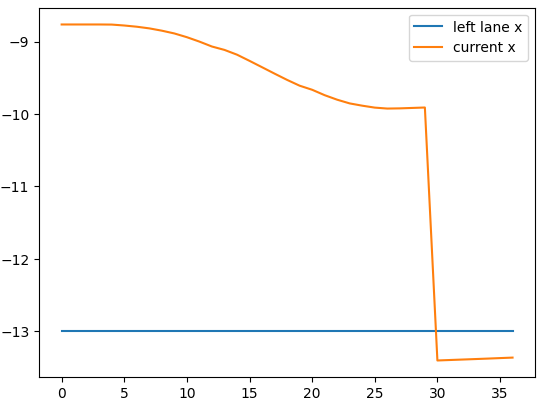
\includegraphics[width=.4\textwidth]{img/pid_controller} }}%
			\qquad
			\subfloat[\centering Lenkwinkel im Laufe der Zeit]{{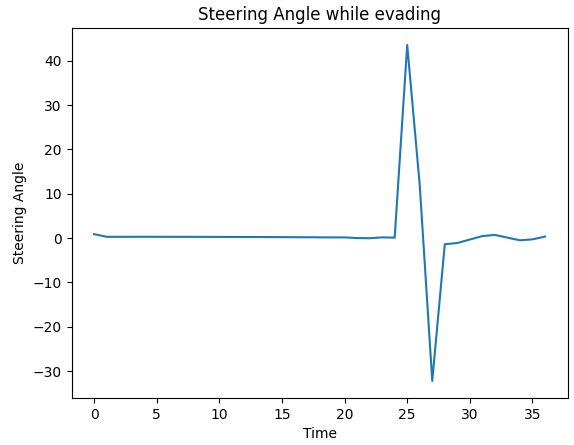
\includegraphics[width=.4\textwidth]{img/steering_angle} }}%
			\caption{Graphische Darstellung eines Ausweichmanövers}%
			\label{fig:manoever}%
		\end{figure}
	\end{itemize}
\end{enumerate}

\section{Testdokumentation}
Die Testdokumentation bildet einen integralen Bestandteil des Entwicklungsprozesses für das Collision Avoidance Assist-System. Sie basiert auf dem zuvor definierten Softwareentwurf und Architektur und enthält eine umfassende Sammlung von Testfällen und -szenarien, die entwickelt wurden, um die Funktionalität, Leistung und Sicherheit des Systems zu überprüfen. Die Tests wurden auf Basis der definierten funktionalen und nicht-funktionalen Anforderungen entworfen, um sicherzustellen, dass das System alle gestellten Anforderungen erfüllt und zuverlässig arbeitet.
\subsection{Use Case \enquote{Forward Collision Warning}}
\textbf{1.1. Testfall: Im kritischen Zustand kommt eine Warnung}
\begin{itemize}
	\item Eingaben
	\begin{itemize}
		\item Fahrer aktiviert das System und fährt mit 60 km/h.
		\item Das vorausfahrende Fahrzeug hat eine Distanz von 36 Metern.
	\end{itemize}
	\item Erwartete Ausgaben
	\begin{itemize}
		\item Das System gibt eine Rückmeldung an Fahrer, dass das System aktiviert wurde.
		\item Das System warnt der Fahrer visuell mit einem gelben Licht, dass das vorausfahrende Fahrzeug nah ist und es eine Kollisionsgefahr besteht.
	\end{itemize}
\end{itemize}
\subsection{Use Case \enquote{Automatic Emergency Braking}}
\textbf{2.1. Testfall: Das vordere Fahrzeug stoppt}
\begin{itemize}
	\item Eingaben
	\begin{itemize}
		\item Fahrer aktiviert das System und fährt mit 60 km/h.
		\item Das vorausfahrende Fahrzeug wurde irgendeinem Grund plötzlich gestoppt und hat eine Distanz von 17 Metern.
	\end{itemize}
	\item Erwartete Ausgaben
	\begin{itemize}
		\item Das System gibt eine Rückmeldung an Fahrer, dass das System aktiviert wurde.
		\item Die Distanz zwischen dem vorausfahrenden Fahrzeug und unserem Fahrzeug ist groß genug, so dass das System in der Lage ist, das Fahrzeug stoppen zu können, ohne Kollisionen zu verursachen.
		\item Das System übernimmt die Kontrolle des Fahrzeugs und wird voll-gebremst.
	\end{itemize}
\end{itemize}
\textbf{2.2. Testfall: Das vorausfahrende Fahrzeug fährt langsamer als uns}
\begin{itemize}
	\item Eingaben
	\begin{itemize}
		\item Fahrer aktiviert das System und fährt mit 60 km/h.
		\item Das vorausfahrende Fahrzeug fährt langsamer als uns.
	\end{itemize}
	\item Erwartete Ausgaben
		\begin{itemize}
		\item Das System gibt eine Rückmeldung an Fahrer, dass das System aktiviert wurde.
		\item Die Distanz zwischen dem vorausfahrenden Fahrzeug und unserem Fahrzeug ist groß genug, so dass das System in der Lage ist, das Fahrzeug verlangsamen zu können, ohne Kollisionen zu verursachen.
		\item Das System übernimmt die Kontrolle des Fahrzeugs und verringert die Geschwindigkeit.
	\end{itemize}
\end{itemize}
\subsection{Use Case \enquote{Automatic Obstacle Avoidance}}
\textbf{3.1. Testfall: Die linke Spur ist frei.}
\begin{itemize}
	\item Eingaben
	\begin{itemize}
		\item Fahrer aktiviert das System und fährt mit 60 km/h.
		\item Das vorausfahrende Fahrzeug wurde irgendeinem Grund plötzlich gestoppt und hat eine Distanz von 15 Metern.
		\item Die Distanz zwischen dem vorausfahrenden Fahrzeug und unserem Fahrzeug ist nicht groß genug zu stoppen, ohne die Kollisionen zu verursachen.
		\item Dem Algorithmus ist angegeben, dass nur die linke Spur frei ist.
	\end{itemize}
	\item Erwartete Ausgaben
	\begin{itemize}
		\item Das System gibt eine Rückmeldung an Fahrer, dass das System aktiviert wurde.
		\item Das System gibt eine Rückmeldung an Fahrer, dass Obstacle Avoidance aktiviert wurde.
		\item Das System übernimmt die Kontrolle und biegt an linke Spur, um Kollision zu vermeiden.
	\end{itemize}
\end{itemize}
\textbf{3.2. Testfall: Die rechte Spur ist frei.}
\begin{itemize}
	\item Eingaben
	\begin{itemize}
		\item Fahrer aktiviert das System und fährt mit 60 km/h.
		\item Das vorausfahrende Fahrzeug wurde irgendeinem Grund plötzlich gestoppt und hat eine Distanz von 15 Metern.
		\item Die Distanz zwischen dem vorausfahrenden Fahrzeug und unserem Fahrzeug ist nicht groß genug zu stoppen, ohne die Kollisionen zu verursachen.
		\item Dem Algorithmus ist angegeben, dass nur die rechte Spur frei ist.
	\end{itemize}
	\item Erwartete Ausgaben
	\begin{itemize}
		\item Das System gibt eine Rückmeldung an Fahrer, dass das System aktiviert wurde.
		\item Das System gibt eine Rückmeldung an Fahrer, dass Obstacle Avoidance aktiviert wurde.
		\item Das System übernimmt die Kontrolle und biegt an rechte Spur, um Kollision zu vermeiden.
	\end{itemize}
\end{itemize}
\textbf{3.3. Testfall: Beide Spuren sind frei.}
\begin{itemize}
	\item Eingaben
	\begin{itemize}
		\item Fahrer aktiviert das System und fährt mit 60 km/h.
		\item Das vorausfahrende Fahrzeug wurde irgendeinem Grund plötzlich gestoppt und hat eine Distanz von 15 Metern.
		\item Die Distanz zwischen dem vorausfahrenden Fahrzeug und unserem Fahrzeug ist nicht groß genug zu stoppen, ohne die Kollisionen zu verursachen.
		\item Dem Algorithmus ist angegeben, dass die beiden Spuren frei sind.
	\end{itemize}
	\item Erwartete Ausgaben
	\begin{itemize}
		\item Das System gibt eine Rückmeldung an Fahrer, dass das System aktiviert wurde.
		\item Das System gibt eine Rückmeldung an Fahrer, dass Obstacle Avoidance aktiviert wurde.
		\item Das System übernimmt die Kontrolle und biegt an die Spur, in der es weniger wahrscheinlich ist, eine andere Kollision zu verursachen.
	\end{itemize}
\end{itemize}
\textbf{3.4. Testfall: Keine Spuren sind frei.}
\begin{itemize}
	\item Eingaben
	\begin{itemize}
		\item Fahrer aktiviert das System und fährt mit 60 km/h.
		\item Das vorausfahrende Fahrzeug wurde irgendeinem Grund plötzlich gestoppt und hat eine Distanz von 15 Metern.
		\item Die Distanz zwischen dem vorausfahrenden Fahrzeug und unserem Fahrzeug ist nicht groß genug zu stoppen, ohne die Kollisionen zu verursachen.
		\item Dem Algorithmus ist angegeben, dass keine der beiden Spuren frei sind.
	\end{itemize}
	\item Erwartete Ausgaben
	\begin{itemize}
		\item Das System gibt eine Rückmeldung an Fahrer, dass das System aktiviert wurde.
		\item Das System gibt eine Rückmeldung an Fahrer, dass Obstacle Avoidance aktiviert wurde.
		\item Es ist dem System bekannt geworden, dass eine Kollision in diesem Fall unvermeidbar ist. Die Richtung, die am wenigsten Schade verursacht wird ausgewählt.
	\end{itemize}
\end{itemize}
\subsection{Testbericht}
Dieser Testbericht dokumentiert die Ergebnisse der durchgeführten Black-Box-Tests für die oben genannten Funktionen des Systems. Die Testfälle wurden gemäß den Hauptszenarien entworfen, um die Funktionalität und die Ausnahmebehandlung des Systems zu überprüfen. Insgesamt wurden in diesem Projekt 7 Black-Box-Tests durchgeführt. 4 Hauptszenarien haben den Test erfolgreich bestanden. 3 Hauptszenarien haben den Test nicht bestanden. Fehler und deren Behebung wurden intern diskutiert und bewertet.
\subsubsection{Zusammenfassung der Ergebnisse}
Im Allgemeinen wurden von verschiedenen Herausforderungen festgestellt. Erstens - wurden manche Funktionen nicht implementiert. Dies geschah bewusst und wurde im Softwareentwurf dokumentiert. Die fehlenden Funktionen werden in der nächsten Softwareauslieferung implementiert und ausgeliefert. Begrenzte Zeit, Fristen und unzureichende Ressourcen für die Installation, Konfiguration und Nutzung von CARLA haben den Entwicklern viel Zeit gekostet. Die wichtigsten Funktionen des Use-Cases funktionieren jedoch wie erwartet und können daher an die Stakeholder ausgeliefert werden. Die fehlenden Teile werden bei der nächsten Auslieferung durch Updates abgedeckt.
\subsubsection{Fazit}
Die Black-Box-Tests haben gezeigt, dass nur grundlegende implementierten Systemfunktionen den Anforderungen entsprechen. Die grundlegenden Tests wurden erfolgreich abgeschlossen aber sie müssen noch verbessert werden, um alle Aspekte der Stakeholder abzudecken.
	%\section{Fazit}
\blindtext[1]
	\subsection{Zusammenfassung}
	\blindtext[2]
	\subsection{Reflexion \& Bewertung der Aufgabenstellung}
	\blindtext[2]
	\subsection{Ausblick}
	\blindtext[4]
	\clearpage
	
	%Römische Seitennummerierung
	\pagenumbering{Roman}
	\setcounter{page}{1}
	
	% ================================
	% Falls nicht verwendet bitte entsprechend auskommentieren
	% ================================
	%Anhang
	%\addsec{Anhang}
	\pagebreak
	
	%Abbildungsverzeichnis
	\listoffigures
	\pagebreak
	
	%Tabellenverzeichnis
	%\listoftables
	\pagebreak

	%Literaturverzeichnis
	%\bibliographystyle{literature/bibtex/IEEEtran}	
	%\bibliography{literature/literature}
	
\end{document}